
\chapter{Results}
\label{sec:org847717f}

In this chapter the simulation results are presented with reference to the aim of the thesis, which was to study the mapping metrics.
Their precision when assessing the mapping quality and their relation with the error amount after mapping.
First, in the \hyperref[sec:org03081b5]{Impact of mapping in the overall circuit error} section we show how the mapping procedure affects the general increment of error.
After that, we analyze the metrics and their correlation with the error increase in the \hyperref[sec:org745344e]{Analysis of the mapping metrics} section.
Finally, in the \hyperref[sec:org19da4a6]{Advice} section, after a regression study, we offer a way to predict the amount of errors a circuit could get depending on the its characteristics.

\section{Impact of mapping in the overall circuit error}
\label{sec:org03081b5}
After the selection of benchmarks in the \href{chapter-4.org}{Benchmarks} section, we started their simulations with the simulation framework.
Not surprisingly, some of the benchmarks either had very long simulation times or were even impossible to simulate in our lab servers.
Most of them had more than ten qubits.
As we mentioned before throughout this thesis, the simulation of quantum systems is computationally exhausting.
As the number of qubits or the longitude of the circuit increases, the harder is to simulate them.
A critical issue in our case, that we need to run multiple simulations in a complex error model.
Therefore, as it can be seen in Tab. \ref{tab:map_selected_benchs}, we aware that the final benchmark selection has a limitation in the number of qubits.
We are also conscious that the percentage of two-qubit gates in the used benchmarks has a majority of values around the 40\%.

\begin{table}[htbp]
\caption{Table of the selected benchmarks to be mapped.}
\centering
\small
\begin{tabular}{lrrr}
\hline
Benchmark & \# qubits & \# gates & two-qubit gates (percentage)\\
\hline
4gt11\(_{\text{82}}\) & 5 & 27 & 0.667\\
4gt12\(_{\text{v1}}\)\(_{\text{89}}\) & 6 & 228 & 0.439\\
4gt4\(_{\text{v0}}\)\(_{\text{72}}\) & 6 & 258 & 0.438\\
4mod5\(_{\text{bdd}}\)\(_{\text{287}}\) & 7 & 70 & 0.443\\
4mod5\(_{\text{v0}}\)\(_{\text{20}}\) & 5 & 20 & 0.500\\
alu\(_{\text{bdd}}\)\(_{\text{288}}\) & 7 & 84 & 0.452\\
alu\(_{\text{v0}}\)\(_{\text{27}}\) & 5 & 36 & 0.472\\
decod24\(_{\text{bdd}}\)\(_{\text{294}}\) & 6 & 73 & 0.438\\
decod24\(_{\text{enable}}\)\(_{\text{126}}\) & 6 & 338 & 0.441\\
graycode6\(_{\text{47}}\) & 6 & 5 & 1.000\\
ham3\(_{\text{102}}\) & 3 & 20 & 0.550\\
hwb4\(_{\text{49}}\) & 5 & 233 & 0.459\\
mod10\(_{\text{176}}\) & 5 & 178 & 0.438\\
mod5adder\(_{\text{127}}\) & 6 & 555 & 0.431\\
mod5d1\(_{\text{63}}\) & 5 & 22 & 0.591\\
mod8\(_{\text{10}}\)\(_{\text{177}}\) & 6 & 440 & 0.445\\
one\(_{\text{two}}\)\(_{\text{three}}\)\(_{\text{v1}}\)\(_{\text{99}}\) & 5 & 132 & 0.447\\
one\(_{\text{two}}\)\(_{\text{three}}\)\(_{\text{v3}}\)\(_{\text{101}}\) & 5 & 70 & 0.457\\
rd32\(_{\text{v0}}\)\(_{\text{66}}\) & 4 & 34 & 0.471\\
sf\(_{\text{274}}\) & 6 & 781 & 0.430\\
sf\(_{\text{276}}\) & 6 & 778 & 0.432\\
sym6\(_{\text{145}}\) & 7 & 3888 & 0.438\\
xor5\(_{\text{254}}\) & 6 & 7 & 0.714\\
\hline
\end{tabular}
\end{table}

\label{tab:map_selected_benchs}

As explained in the \href{chapter-4.org}{Analysis Framework} section, after running the benchmarks the results obtained are the fidelity, the probability of success and the Quantum Volume.
We also extract other metrics like the number of SWAPs added and the depth of the circuits, between others.
To match the three router algorithms developed in our group (see \href{chapter-3.org}{Mapping model}) we compiled the list of benchmarks with four different configurations.
One per router and another one without mapping the algorithms to any device.
For a fair comparison, the non-mapped configuration make the compiler to decompose the circuit gates in the SC-17 gate set (see Fig. \ref{fig:decompositions}).
We also tried different configurations regarding the decoherence time and the error rates in order to study the mappers in different error regimes.


The framework results immediately confirmed that the mapping procedure affects the error amount in the quantum system.
In Fig. \ref{fig:f_diff_bar_plot} we highlight the difference in fidelity of some benchmarks before and after being mapped.
The mapped data we plot comes from the router \texttt{minextendrc}.
We can see how the fidelity is smaller for long circuits -- like \texttt{sf\_274} or \texttt{mod5adder\_127} -- than for the short ones -- \texttt{graycode6\_47} or \texttt{xor5\_254}.
We show the exact result values in \href{appendix-1.org}{Appendix A}.

\begin{figure}[htbp]
\centering
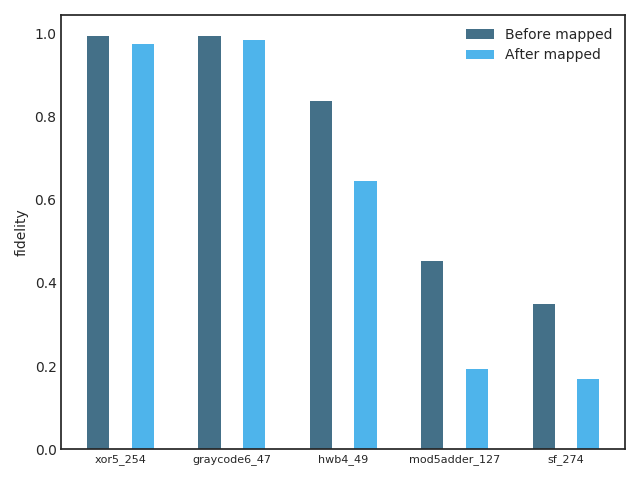
\includegraphics[width=0.7\textwidth]{figures/f_diff_bar_plot.png}
\caption{\label{fig:f_diff_bar_plot}
Difference of fidelities before and after mapping with the \texttt{minextendrc} router for five different benchmarks.}
\end{figure}
In Fig. \ref{fig:infid_percentage_depth_before_mapping} we can see [explain the points that I'm plotting and the selection of them as well as what we are trying to show]
I WANT TO FIND A BETTER WAY TO SHOW THIS INSIGHTS BEFORE I EXPLAIN THEM

\begin{itemize}
\item In order to get this figure we filter fidelity. Only f>0.5 is plot
\item Infidelity: \(\frac{f_a - f_b}{1 - f_b}\)
\item Depth is the depth before mapping
\item We decided to see it like this in order to cluster the same benchmark mapped in different ways
\item We can conclude that the mapper quality is critical for benchmarks with small depth before being mapped, but for long circuits the mapper quality gets diminished. This means that simple and, therefore, faster mappers can be implemented for long circuits making possible the mapping on the fly, for instance
\end{itemize}

\begin{figure}[htbp]
\centering
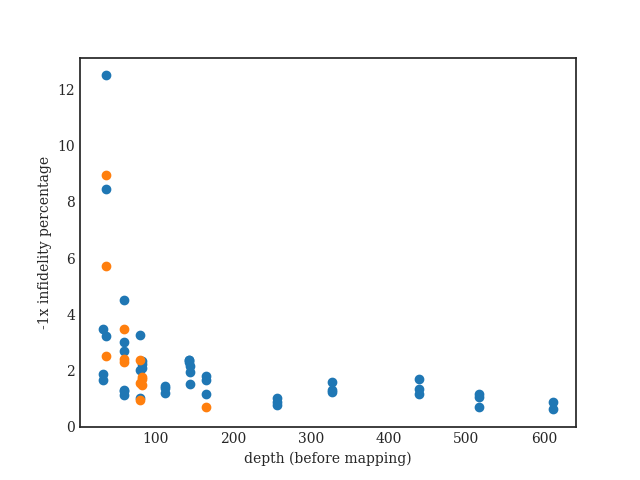
\includegraphics[width=0.7\textwidth]{figures/infid_percentage_depth_before_mapping.png}
\caption{\label{fig:infid_percentage_depth_before_mapping}
}
\end{figure}

We can inherit that the longer the circuit is before being mapped, the less impact the mapping will have over it.
In this case, even before mapped, the circuit is going to have a low fidelity or probability of success.
And after mapped, that situation does not change that much.

\section{Analysis of the mapping metrics}
\label{sec:org745344e}
In this section we evaluate the behaviour and quality of the mapping metrics.
From the classical ones -- number of SWAPs and depth -- to the ones we proposed -- fidelity, probability of success and Quantum Volume.


First we analyze the probability of success and fidelity correlation.
As expected, our experiments prove that both metrics are highly linearly correlated.
We also appreciated the fact that the probability of success is always higher than the fidelity.
This could suggest that the measurement is 'correcting' circuit errors colliding the state in the correct result, although this could be caused by the fact that our algorithms are deterministic.
While comparing the results with different decoherence times, we noticed as well that the more errors introduced in the system, the closer are the values of the probability of success and fidelity.

In Fig. \ref{fig:f_ps_correlation_with_meas_error} we plot the results of the framework in terms of probability of success and fidelity. 
Each dot is a different benchmark configuration and the colors represent different decoherence times in the simulation, blue for 30 \(\mu s\) and orange for 10 \(\mu s\).
The figure highlights the linear correlation as well as the line bias proving the fact that the probability of success is always higher than the fidelity.
It can be seen that the inclination and bias of the fitting line changes depending on the decoherence time.
Showing that, the higher amount of errors in the system, the more diagonal the fitting line gets.
The cluster that appears between the 0.9 and 1.0 values is due to the amount of simple benchmarks in the selection, as we previously mentioned.

\begin{figure}[htbp]
\centering
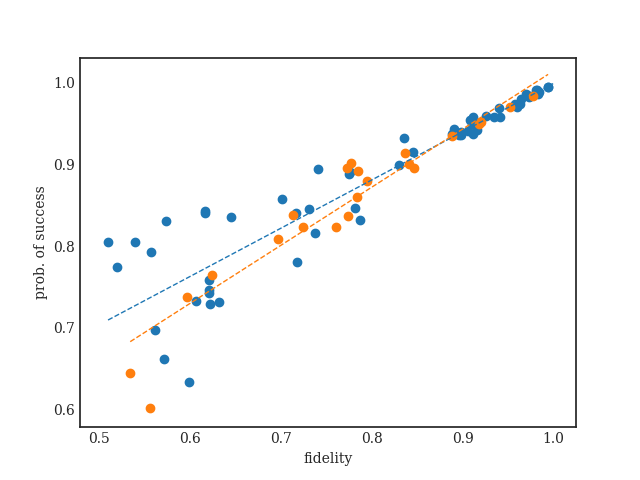
\includegraphics[width=0.7\textwidth]{figures/f_ps_correlation_with_meas_error.png}
\caption{\label{fig:f_ps_correlation_with_meas_error}
Correlation between fidelity and probability of success for two different decoherence times}
\end{figure}



We use the Pearson correlation to measure which metric is the most correlated one with fidelity and probability of success.
As it can be seen in the Pearson values (Tab. [REFER TO TAB]) the metric most correlated is the number of two-qubit gates.
These results hold the fact that the quality of the mapping depends on the longitude of the targeted circuit, making crucial the mapping quality for small benchmarks.

[CORRELATION TABLE]

Quantum's Volume small lack of correlation can be attributed to the imprecise formula that we chose to calculate it.
Given that this was only a preliminary attempt to include the Quantum Volume as mapping metric it is hardly surprising that the results are not directly correlating it with the mapping quality.

The results of the main mapping metrics against fidelity are depicted in Fig. \ref{fig:f_metrics_correlation}.
As in previous plots, we show the results for two different decoherence times, 30 \(\mu s\) (blue dots) and 10 \(\mu s\) (orange dots).
We observe that, for all the cases, the fidelity decreases with an inverse exponential behaviour.

\begin{figure}[htbp]
\centering
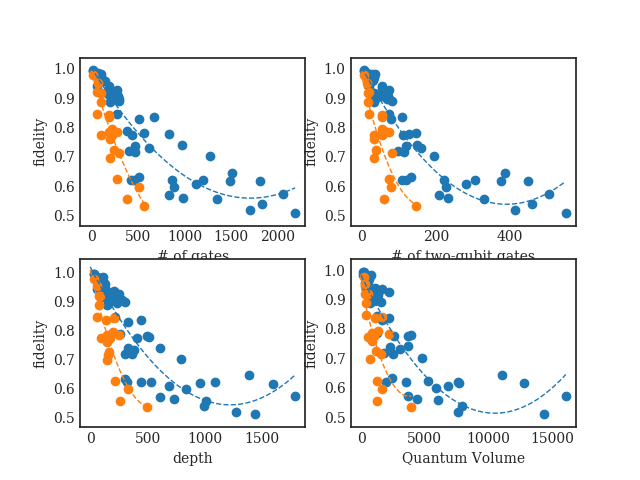
\includegraphics[width=\textwidth]{figures/f_metrics_correlation.png}
\caption{\label{fig:f_metrics_correlation}
Correlation between fidelity and the mapping metrics.}
\end{figure}

The correlation between the probability of success and the other metrics can be see in Fig. \ref{fig:ps_metrics_correlation}.
As with the study on fidelity correlation we plot two decoherence times, 30 \(\mu s\) (blue) and 10 \(\mu s\) (orange).
We also observe a decreasing behaviour, although the shape is not as clear as in the case of fidelity.
This could be provoked by the final error added by the measurement gate and by the fact that, most of the times, the measurement is correcting the wrong solutions.

\begin{figure}[htbp]
\centering
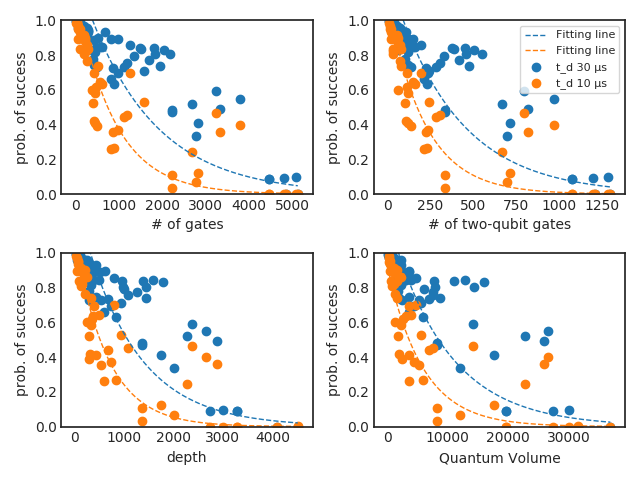
\includegraphics[width=\textwidth]{figures/ps_metrics_correlation.png}
\caption{\label{fig:ps_metrics_correlation}
Correlation between probability of success and the mapping metrics.}
\end{figure}

We can also see in both figures that, as announced before, there is a cluster of benchmarks with high fidelity and high probability of success.
This happens because of the high concentration of small benchmarks, due to the simulation difficulties.
On the contrary, the rest of the values are a bit sparsed.

\section{Advice}
\label{sec:org19da4a6}
After analyzing the correlation between metrics we begin the regression analysis.
We aim to understand the behaviour of our data and be able to predict the fidelity or the probability of success given the circuit parameters and the error rates.

Our regression model is based on a double regression model.
First our model learns and predicts from the samples with Support Vector Machines (SVM) using as kernel the Radial Basis Function (RBF) and then, with those predictions we feed a second regression model in order to shaped the first analysis.
The SVM model was chosen because it is one of the most practical, rapid and ergonomic ways to commit a regression model.
The flexibility of the regression model is critical in our case due to the non-linear aspect of the data.
For the second regression model we use different, much simpler, regression algorithms with the intention to find the model that fits the data the best.
In the Fig. \ref{fig:f_metrics_correlation} and \ref{fig:ps_metrics_correlation} we present fitting lines predicted after the regression model we used.

\subsection{Fidelity}
\label{sec:org50cea58}

For the model between the metrics and the fidelity we opted for a [POLYNOMIAL/EXPONENTIAL] regression model as the second regression algorithm.

\subsection{Probability of success}
\label{sec:org2f1ace2}

In the case of the probability of success model we opted for a [LINEAL] regression mode for the second regression process.
